\chapter{Goby-Acomms}\label{chap:acomms}
\MakeShortVerb{\!} % makes !foo! == !foo!

\section{Introduction}

\subsection{Problem}
Acoustic communications are highly limited in throughput. Thus, it is unreasonable to expect ``total throughput'' of all communications data. Furthermore, even if total throughput is achievable over time, certain messages have a lower tolerance for delay (e.g. vehicle status) than others (e.g. CTD sample data). 

Also, in order to make the best use of this available bandwidth, messages need to be compacted to a minimal size before sending (effective encoding). To do this, Goby-Acomms provides an interface to the Dynamic Compact Control Language (DCCL\footnote{the name comes from the original CCL written by Roger Stokey for the REMUS AUVs, but with the ability to dynamically reconfigure messages based on mission need. If desired, DCCL can be configured to be backwards compatible with a CCL network using CCL message number 32}) encoder/decoder. 

For the interested reader, the publications listed in the Developers' documentation \cite{goby-doc} give a more in-depth look at the problem.

\subsection{Goby contributions to the solution}

Goby is hardly a complete solution to this problem, but it's a start. It provides four key components (listed in order from closest to the application to closest to the physical link) intended to address the limits of traditional networking systems in light of the extreme bandwidth and latency constraints of underwater links:

\begin{enumerate}
\item The \textbf{Dynamic Compact Control Language (DCCL)} (section \ref{sec:dccl}) is a marshalling (or synonymously serialization) scheme that creates highly compressed small messages suitable for sending over links with very low maximum transmission units (order of 10s to 100s of bytes) such as typical underwater acoustic modems. DCCL  provides greater efficiency (i.e. smaller messages) than existing marine (CCL, Inter-Module Communication) and non-marine (Google Protobuf, ASN.1, boost::serialization, etc.) techniques by pre-sharing all structural information and bounding message fields to minimum and maximum values (which then create messages of any bit size, not limited by integer multiples of octets such as int16, int32, etc.). The DCCL structure language is independent of a given programming language and provides compile-time type safety and syntax checking, both of which are important for fielding complex robotic systems. Finally, DCCL is extensible to allow user-provided source encoders for any given field or message type.
\item The transport layer of Goby-Acomms provides time dynamic priority queuing (\textbf{Goby-Queue}, section \ref{sec:queue}). In our experience, acoustic links on fielded vehicles have been typically run at over-capacity; that is, there are more data to send than will ever be send over the link. Thus, the data that are to be sent must be chosen in some fashion. Historically, priority queues are widely used to send more valuable data first. However, different types of data also have different time sensitivities, which Goby-Queue recognizes via the use of a (clock time based) time-to-live parameter. Finally, the demand for a given type of data can increase over time since last receiving a message of that type. Goby-Queue extends the traditional priority queue concept to balance these various demands and send the most valuable data under this set of metrics.
\item Acoustic modems such as the WHOI Micro-Modem do not provide any shared access of the acoustic channel. Coordinating shared access can be accomplished by assigning slots of time in which each vehicle can transmit, which is the time-division multiple access (TDMA) flavor of medium access control (MAC). The \textbf{Goby-Acomms acoustic MAC (AMAC), section \ref{sec:amac}} extends the basic TDMA idea to include passive (i.e. no data overhead) auto-discovery of vehicles in a small, equally time-shared network. Thus, AMAC simplifies the amount of pre-deployment configuration required to configure small networks of AUVs.
\item The \textbf{Goby ModemDriver} (section \ref{sec:driver}) provides an abstract interface for acoustic modems (and other ``slow link'' devices, such as satellite modems), as there is no standard for interfacing to such devices. Many acoustic modems provide functionality beyond the strict definition of a modem (which is defined as sending data from one point to another). Examples of these extra features include navigation (long base line or LBL, ultra-short base line or USBL) and ranging measurements (``pings''). Goby ModemDriver allows an application intent only on transmitting data to operate on any implemented modem without concerning itself with the details of that device. On the other hand, if the application needs to use some of the extra features, it can do so via a set of well-defined extensions. 
\end{enumerate}

These components are loosely coupled. For example, it is possible to use the ModemDriver (with or without AMAC) to send encoded messages of any origin. You can also use DCCL without any of the other components. However, Queue requires DCCL (it does not queue other types of messages). Thus, you can design systems using only one, several, or all of the components of Goby, as you need and see fit.


\section{Dynamic Compact Control Language: DCCL} \label{sec:dccl}

DCCL allows you to take object based ``messages'' (similar to C structs) defined in the Google Protocol Buffers language and extend them to be more strictly bounded. It provides a set of default encoders for these bounded Protocol Buffers messages (now called DCCL messages) to provide a more minimal encoding than the default Protocol Buffers encoding (which is reasonably decent already, but still has too much overhead for extremely slow links). 

Thus, broadly speaking, DCCL provides an alternative (more compact and extensible) encoding scheme for Google Protocol Buffers, at some cost of additional development time and the requirement that the sender and receiver share the exact .proto definition file (which the normal protobuf encoder does not require). In our experience, this extra effort is worth it for acoustic (and other ``very slow link'' networks, such as satellite).

\subsection{Configuration: DCCLConfig}

Configuration of individual DCCL messages (the vast majority of DCCL configuration) is done within the .proto definition. All the non-message specific available configuration for !goby::acomms::DCCLCodec! is given in its TextFormat form as:

\boxedverbatiminput{@RELATIVE_CMAKE_CURRENT_SOURCE_DIR@/includes/dccl_config.pb.cfg}
\resetbvlinenumber

\begin{itemize}
\item !crypto_passphrase!: If provided, this preshared key is used to encrypt the body of all messages using AES (Rijndael) encryption. Omit this field to turn off encryption. Note that the contents of messages received by nodes with the wrong encryption key are undefined, and such failure is not currently detected.
\end{itemize}

\subsection{Configuration: Designing DCCL messages using Protocol Buffers Extensions}


%\begin{figure}
%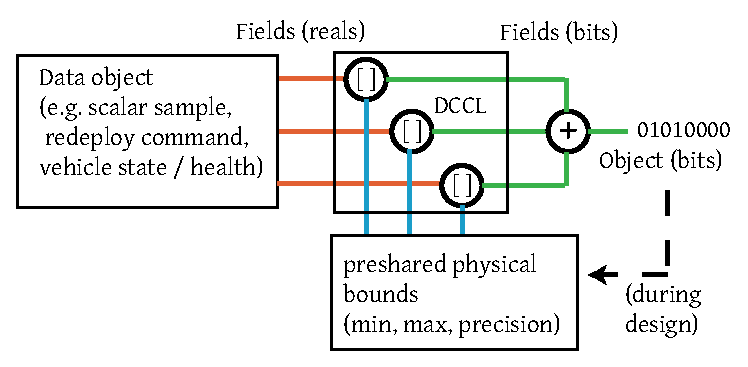
\includegraphics[scale=1]{dccl-schematic.eps} 
%\end{figure}


A full guide to designing DCCL messages is given at \url{http://gobysoft.com/doc/2.0/acomms_dccl.html} along with a full list of the DCCL extensions to the Google Protobuf !MessageOptions! (i.e. !(dccl.msg).*!) and !FieldOptions! (i.e. !(dccl.field).*!). Therefore, we will not replicate that information here. However, we will give a broad overview of the DCCL configuration.

DCCL messages are protobuf messages with ``invisible'' extensions. By ``invisible,'' we mean that DCCL messages can be compiled by the standard protobuf compiler (!protoc!) without requiring the Goby-Acomms library. This allows DCCL messages to be shared with users that do not need the functionality of DCCL (e.g. are only using traditional IP networks), but need to communicate with groups that need the additional compression afforded by DCCL. The goal is to break down the barriers for using acoustic links on robotic systems, while still maintaining the efficiency necessary for effective use of these highly restricted links.

A simple, but realistic, protobuf message might look like this:

\begin{boxedverbatim}
package example;

message MinimalStatus
{ 

  required double time = 1;
  required int32 source = 2;
  required int32 dest = 3;
  required double x = 4;
  required double y = 5;  
  required double depth = 6;
} 
\end{boxedverbatim}
\resetbvlinenumber

The field numbers (e.g. 1 in !time = 1!) are used by the default protobuf encoding (but not by DCCL) to allow backwards compatibility of messages. DCCL requires that both sender and receiver have the identical message definition (.proto file), so for our purpose you just need to make sure no two fields share the same field number. These numbers have no effect in the DCCL encoding.

\textit{A priori}, we know certain physical bounds on the message fields. These can be conservative (if a field goes out-of-bounds, the receiver sees it as empty; that is, !.has_field() == false!), but even conservative bounds will often make a field consume far fewer bytes than the system equivalent. 

Integer (!(u)int32!, !(u)int64!) fields take a !max! and !min! value\footnote{the DCCL bounds must be a subset of the system type's bounds}, and DCCL creates the smallest (bit-sized) integer than can hold that value. For reals (!float! and !double!), an additional !precision! value is provided: this represents the number of decimal digits of precision to preserve (negative values are also allowed). Thus, !precision=1! means round to the nearest tenth, !precision=-2! means round to the nearest hundred.

Booleans (!bool!) and enumerations (!enum!) are automatically bounded their nature, and require no additional configuration. Strings (!string!) (which are generally discouraged on an acoustic link since they tend to be sparse) are bounded by a maximum length. Similarly, !bytes! are pre-encoded data that are passed through unmodified in DCCL. Applying these bounds to the example message above (along with the required .proto file imports) yields:

\begin{boxedverbatim}
import "goby/acomms/protobuf/dccl_option_extensions.proto";

package example;

message MinimalStatus
{ 
  option (dccl.msg).id = 21;
  option (dccl.msg).max_bytes = 10;

  required double time = 1 [(dccl.field).codec="_time",
                            (dccl.field).in_head=true];
  
  required int32 source = 2 [(dccl.field).max=31,
                             (dccl.field).min=0,
                             (dccl.field).in_head=true];

  required int32 dest = 3 [(dccl.field).max=31,
                           (dccl.field).min=0,
                           (dccl.field).in_head=true];
  
  required double x = 4 [(dccl.field).max=10000,
                         (dccl.field).min=-10000,
                         (dccl.field).precision=1];
  
  required double y = 5 [(dccl.field).max=10000,
                         (dccl.field).min=-10000,
                         (dccl.field).precision=1];
  
  required double depth = 6 [(dccl.field).max=6400,
                             (dccl.field).min=0,
                             (dccl.field).precision=-1];
} 
\end{boxedverbatim}
\resetbvlinenumber

The option "!in_head!" tags the field as belonging in the user header. The only distinction between the header and body of a DCCL message is for encryption: the body is encrypted but the header is not (it is used as the nonce). The option !codec! allows a different DCCL codec to be used than the default for that field type (!_time! is a codec that encodes time of day to the nearest second assuming that messages are received within 12 hours of transmission). If you wish to write custom encoders, see the !DCCLTypedFixedFieldCodec! class in the Developers' documentation.

\section{Time dependent priority queuing: Queue} \label{sec:queue}

Goby-Queue manages a queue for each DCCL message. When it is prompted by data by the modem, it has a priority "contest" between the queues. the queue with the current highest priority (as determined by the !value_base! and !ttl! fields) is selected. The next message in that queue is then provided to the modem to send. For modem messages with multiple frames per packet, each frame is a separate contest. Thus a single packet may contain frames from different
 queues (e.g. a rate 5 PSK packet has eight 256 byte frames. frame 1 might grab a STATUS message since that has the current highest queue. then frame 2 may grab a BTR message and frames 3-8 are filled up with CTD messages (e.g. STATUS is in blackout, BTR queue is empty)). See \url{http://gobysoft.com/doc/2.0/acomms_queue.html} for more information.

\subsection{Configuration: QueueManagerConfig}

The configuration options for !goby::acomms::QueueManager! are:

\boxedverbatiminput{@RELATIVE_CMAKE_CURRENT_SOURCE_DIR@/includes/queue_config.pb.cfg}
\resetbvlinenumber

\begin{itemize}
\item !modem_id!: A unique integer value for this particular vehicle (like a MAC address). Should be as small as possible for optimal bounding of the source and destination fields of the message. 0 is reserved for broadcast (analogous to 255.255.255.255 for IPv4).
\item !message_entry!: Configures the QueueManager to queue this DCCL type:
\begin{itemize}
\item !protobuf_name!: String representing the DCCL message to manipulate. Messages are named the same as !google::protobuf::Descriptor::full_name()!, which is the !package! followed by the message name, separated by dots: e.g. ``example.MinimalStatus'' for the message shown in Section \ref{sec:dccl}.
\item !ack!: Whether an acoustic acknowledgment should be requested for messages sent from this queue. If !ack! is true, messages will not be dequeued until a positive !ack! is received (or it expires due to exceeding the !ttl!).
\item !blackout_time!: Minimum number of seconds allowed between sending messages from this queue.
\item !max_queue!: Allowed size of the queue before overflow. If !newest_first! is true, the oldest elements are removed upon overflow, otherwise the newest elements are. 0 is a special value signifying infinity (no maximum).
\item !newest_first!: true	(true=FILO, false=FIFO) whether to send newest messages in the queue first (FILO) or not (FIFO).
\item !ttl!: the time in seconds a message lives after its creation before being discarded. This time-to-live also factors into the growth in priority of a queue. see !value_base! for the main discussion on this. 0 is a special value indicating infinite life (i.e. !ttl! = 0 is effectively the same as !ttl! = $\infty$)
\item !value_base!: base priority value for this message queue. priorities are calculated on a request for data by the modem (to send a message). The queue with the highest priority (and isn't in blackout) is chosen. The actual priority ($P$) is calculated by $P(t) = V_{base} \frac{(t-t_{last})}{ttl}$ where $V_{base}$ is the value set here, $t$ is the current time (in seconds), $t_{last}$ is the time of the last send from this queue, and $ttl$ is the !ttl! option. Essentially, a message with low !ttl! will become effective quickly again after a sent message (the priority line grows faster).
\item !manipulator!: One or more manipulators to apply to the queuing of this message.
\begin{itemize}
\item !NO_MANIP!: A do nothing (noop) manipulator. Same as omitting this field.
\item !NO_QUEUE!: Do not queue this message when generated on this node (but messages will still be received (dequeued).
\item !NO_DEQUEUE!: Do not dequeue (receive) this message on this node (but messages will be queued). When both !NO_QUEUE! and !NO_DEQUEUE! are set, there isn't much point to having the message loaded at all.
\item !LOOPBACK!: Dequeue all instances of this message immediately upon queuing. The message is still queued and sent to its addressed destination. Often used with !PROMISCUOUS!.
\item !ON_DEMAND!: A special (advanced) feature where QueueManager assumes this queue is always full and asks for data immediately from the application upon request from the modem side. Useful for ensuring time sensitive data does not get stale.
\item !LOOPBACK_AS_SENT!: Like loopback, but rather than dequeuing upon queuing, this manipulator dequeues a copy locally upon a data request from the modem. Often used with !PROMISCUOUS!.
\item !PROMISCUOUS!: Dequeue all messages of this type even if this !modem_id! does not match the destination address.
\item !NO_ENCODE!: Same as !NO_QUEUE!, provided for backwards compatibility with Goby v1.
\item !NO_DECODE!: Same as !NO_DEQUEUE!, provided for backwards compatibility with Goby v1.
\end{itemize}
\item role: allows the assignment of a field in the DCCL message to a particular role. This takes the place of a fixed header that strictly hierarchical protocols might use. 
\begin{itemize}
\item !type!: the type of this role. Valid values are !SOURCE_ID! (which represents the source address of this message), !DESTINATION_ID! (the destination address of this message), !TIMESTAMP! (the time this message was created: used for the !ttl! calculation).
\item !setting!: how is the value of this role obtained: !FIELD_VALUE! (read this role's value from the message field given by !field!) or !STATIC! (read this value from this configuration's !static_value! field).
\item !field!: If !setting == FIELD_VALUE!, the field name (e.g. !dest!) in the message whose contents should be used for in this role. Do not set this if using !setting == STATIC!
\item !static_value!: The static value to use for !setting == STATIC!. Has no effect if !setting == FIELD_VALUE!.
\end{itemize}
\end{itemize}
\item !on_demand_skew_seconds!: (Advanced) this sets the number of seconds before data encoded on demand are considering stale and thus must be demanded again with the signal !QueueManager::signal_data_on_demand!. Setting this to 0 is unadvisable as it will cause many calls to !QueueManager::signal_data_on_demand! and thus waste CPU cycles needlessly encoding.
\item !minimum_ack_wait_seconds!: (Advanced) how long to wait for an acknowledgment before resending the same data.
\end{itemize}

For example, to queue the message given in Section \ref{sec:dccl}, the following snippet could suffice:

\begin{boxedverbatim}
message_entry {
  protobuf_name: "example.MinimalStatus"
  ack: false
  blackout_time: 30
  max_queue: 1
  newest_first: true
  ttl: 900
  value_base: 0.5
  role { type: DESTINATION_ID  field: "dest"   }
  role { type: SOURCE_ID       field: "source" }
  role { type: TIMESTAMP       field: "time"   }
}
\end{boxedverbatim}
\resetbvlinenumber

\section{Time Division Multiple Access (TDMA) Medium Access Control (MAC): AMAC} \label{sec:amac}

The AMAC unit uses time division (TDMA) to attempt to ensure a collision-free acoustic channel.

AMAC supports two variants of the TDMA MAC scheme: centralized and decentralized. As the names suggest, Centralized TDMA (!type: MAC_POLLED!) involves control of the entire cycle from a single master node, whereas each node's respective slot is controlled by that node in Decentralized TDMA. Within decentralized TDMA, Goby supports a fixed (preprogrammed) cycle (!type: MAC_FIXED_DECENTRALIZED!) that can be updated by the application. The autodiscovery mode (!type: MAC_AUTO_DECENTRALIZED!) supported in version 1 is no longer provided in version 2. To disable the AMAC, use (!type: MAC_NONE!). See \url{http://gobysoft.com/doc/2.0/acomms_mac.html} for more details.

\subsection{Configuration: MACConfig}

The !goby::acomms::MACManager! is basically a !std::list<ModemTransmission>!. Thus, its configuration is primarily such an initial list of these !slot!s. Since !ModemTransmission! is extensible to handle different modem drivers, the AMAC configuration is also automatically extended. Some fields in !ModemTransmission! do not make sense to configure !goby::acomms::MACManager! with, so these are omitted here:

\boxedverbatiminput{@RELATIVE_CMAKE_CURRENT_SOURCE_DIR@/includes/mac_config.pb.cfg}
\resetbvlinenumber


Further details on these configuration fields: 
\begin{itemize}
\item !type!: type of Medium Access Control. See \url{http://gobysoft.com/doc/2.0/acomms_mac.html#amac_schemes} for an explanation of the various MAC schemes.
\item !slot!: use this repeated field to specify a manual polling or fixed TDMA cycle for the  !type: MAC_FIXED_DECENTRALIZED! and  !type: MAC_POLLED!. 
\begin{itemize}
\item !src!: The sending !modem_id! for this slot. Setting both src and dest to 0 causes AMAC to ignore this slot (which can be used to provide a blank slot).
\item !dest!: The receiving !modem_id! for this slot. Omit or set to -1 to allow next datagram to set the destination.
\item !rate!: Bit-rate code for this slot (0-5). For the WHOI Micro-Modem 0 is a single 32 byte packet (FSK), 2 is three frames of 64 bytes (PSK), 3 is two frames of 256 bytes (PSK), and 5 is eight frames of 256 bytes (PSK).
\item !type!: Type of transaction to occur in this slot. If !DRIVER_SPECIFIC!, the specific hardware driver governs the type of this slot (e.g. ![micromodem.protobuf.type]!: !MICROMODEM_MINI_DATA!. 
\item !slot_seconds!: The duration of this slot, in seconds.
\item !unique_id!: Integer field that can optionally be used to identify certain types of slots. For example, this allows integration of an in-band (but otherwise unrelated) sonar with the modem MAC cycle.
\end{itemize} 
\end{itemize} 

Relevant extensions of !goby::acomms::protobuf::ModemTransmission! for the WHOI Micro-Modem driver (!DRIVER_WHOI_MICROMODEM!):
\begin{itemize}
\item !slot!
\begin{itemize}
\item ![micromodem.protobuf.type]!: Type of transaction to occur in this slot. This value is only used if !type == DRIVER_SPECIFIC!. Valid values include: !BASE_TYPE! (use the type given in !type! above), !MICROMODEM_TWO_WAY_PING! (!$CCMPC!, !MICROMODEM_REMUS_LBL_RANGING! (!$CCPDT!), !MICROMODEM_NARROWBAND_LBL_RANGING! (!$CCPNT!), !MICROMODEM_MINI_DATA! (!$CCMUC!).
\item ![micromodem.protobuf.narrowband_lbl]!: Narrowband long-baseline configuration. These are merged with any global settings given in the ModemDriver configuration (Section \ref{sec:driver}), with the values set here taking precedence.
\item ![micromodem.protobuf.remus_lbl]!: REMUS long-baseline configuration. These are merged with any global settings given in the ModemDriver configuration (Section \ref{sec:driver}), with the values set here taking precedence.
\end{itemize} 
\end{itemize} 

Several examples:
\begin{itemize}
\item Continous uplink from node 2 to node 1 with a 15 second pause between datagrams (this is node 1's configuration; it is the same for node 2 except for !modem_id = 2!):
\begin{boxedverbatim}
modem_id: 1
type: MAC_FIXED_DECENTRALIZED
slot { src: 2  dest: 1  type: DATA  slot_seconds: 15 }
\end{boxedverbatim}
\resetbvlinenumber
\item Equal sharing for three vehicles (destination governed by next data packet):
\begin{boxedverbatim}
modem_id: 1 # 2 or 3 for other vehicles
type: MAC_FIXED_DECENTRALIZED
slot { src: 1  type: DATA  slot_seconds: 15 }
slot { src: 2  type: DATA  slot_seconds: 15 }
slot { src: 3  type: DATA  slot_seconds: 15 }
\end{boxedverbatim}
\resetbvlinenumber
\item Three vehicles with both data and WHOI Micro-Modem two-way ranging (ping):
\begin{boxedverbatim}
modem_id: 1 # 2 or 3 for other vehicles
type: MAC_FIXED_DECENTRALIZED
slot { src: 1  type: DATA  slot_seconds: 15 }
slot { 
  src: 1
  dest: 2
  type: DRIVER_SPECIFIC 
  [micromodem.protobuf.type]: MICROMODEM_TWO_WAY_PING
  slot_seconds: 5
}
slot { 
  src: 1
  dest: 3
  type: DRIVER_SPECIFIC 
  [micromodem.protobuf.type]: MICROMODEM_TWO_WAY_PING
  slot_seconds: 5
}
slot { src: 2  type: DATA  slot_seconds: 15 }
slot { src: 3  type: DATA  slot_seconds: 15 }
\end{boxedverbatim}
\resetbvlinenumber
\item One vehicle interleaving data and REMUS long-base-line (LBL) navigation pings:
\begin{boxedverbatim}
modem_id: 1
type: MAC_FIXED_DECENTRALIZED
slot { src: 1  type: DATA  slot_seconds: 15 }
slot { 
  src: 1
  dest: 2
  type: DRIVER_SPECIFIC 
  [micromodem.protobuf.type]: MICROMODEM_REMUS_LBL_RANGING
  [micromodem.protobuf.remus_lbl] {
    enable_beacons: 0xf   # enable all four: b1111
    turnaround_ms: 50
    lbl_max_range: 500 # meters
  }
  slot_seconds: 5
}
\end{boxedverbatim}
\resetbvlinenumber
\end{itemize}

\section{Abstract Acoustic (or other slow link) Modem Driver: ModemDriver} \label{sec:driver}

The ModemDriver unit provides a common interface to any modem capable of sending datagrams. It currently supports the WHOI Micro-Modem acoustic modem, UDP over the Internet, and is extensible to other acoustic (or slow link) modems. More details on the ModemDriver are available here: \url{http://gobysoft.com/doc/2.0/acomms_driver.html}.

\subsection{Configuration: DriverConfig}

Base driver configuration:

\boxedverbatiminput{@RELATIVE_CMAKE_CURRENT_SOURCE_DIR@/includes/driver_config.pb.cfg}
\resetbvlinenumber

\begin{itemize}
\item !modem_id!: A unique integer value for this particular vehicle (like a MAC address). Should be as small as possible for optimal bounding of the source and destination fields of the message. 0 is reserved for broadcast (analogous to 255.255.255.255 for IPv4).
\item !connection_type!: How the modem is attached to this computer. Some of the drivers do not use this connection. Valid options: !CONNECTION_SERIAL! (uses a serial connection, e.g. !/dev/ttyS0!), !CONNECTION_TCP_AS_CLIENT! (connect using TCP where this application is a client, and the modem is a server), !CONNECTION_TCP_AS_SERVER! (connect using TCP where this application is a server, and the modem is a client).
\item !line_delimiter!: A string representing the ``end-of-line'' of each message from the modem.
\item !serial_port!: Only for !CONNECTION_SERIAL!, the name of the serial port on this machine.
\item !serial_baud!: Only for !CONNECTION_SERIAL!, the baud rate to use when talking to the modem.
\item !tcp_server!: Only for !CONNECTION_TCP_AS_CLIENT!, the IP address or domain name of the modem TCP server.
\item !tcp_port!: For !CONNECTION_TCP_AS_CLIENT!, the port to connect to on !tcp_server!; for !CONNECTION_TCP_AS_SERVER!, the port to bind on.
\end{itemize} 

Extensions for the WHOI Micro-Modem (!DRIVER_WHOI_MICROMODEM!):
\boxedverbatiminput{@RELATIVE_CMAKE_CURRENT_SOURCE_DIR@/includes/driver_mmdriver.pb.cfg}
\resetbvlinenumber

\begin{itemize}
\item ![micromodem.protobuf.Config.reset_nvram]!: If true, reset all the modem's configuration settings at startup (before applying those specified in !nvram_cfg!). In general, it is a good idea to set this to true so that the modem's NVRAM (configuration) state is known.
\item ![micromodem.protobuf.Config.nvram_cfg]!: This repeated field specifies an NVRAM configuration sentence to send. For example, to set !$CCCFG,DTO,10!, use ``DTO,10'' as the value for this field. %$
\item ![micromodem.protobuf.Config.nvram_cfg]!: You must omit this in all cases except when using a Hydroid Buoy which uses a modified talker to communicate with the Micro-Modem. In that case, set this to the Buoy identification number.
\item ![micromodem.protobuf.Config.narrowband_lbl]!: Default configuration used for each !MICROMODEM_NARROWBAND_LBL_RANGING! transmission. Overwritten by any settings also specified in the AMAC configuration. See \url{http://gobysoft.com/doc/2.0/acomms_driver.html} for the details of these fields.
\item ![micromodem.protobuf.Config.remus_lbl]!: Default configuration used for each !MICROMODEM_REMUS_LBL_RANGING! transmission. Overwritten by any settings also specified in the AMAC configuration. See \url{http://gobysoft.com/doc/2.0/acomms_driver.html} for the details of these fields.
\item ![micromodem.protobuf.Config.mm_version]!: Micro-Modem major version. Only Micro-Modem 1 is currently supported (and Micro-Modem 2 in backwards-compatible mode). Thus, currently, this field should always be 1.
\end{itemize} 


Extensions for the example driver (!DRIVER_ABC_EXAMPLE_MODEM!):
\boxedverbatiminput{@RELATIVE_CMAKE_CURRENT_SOURCE_DIR@/includes/driver_abc_driver.pb.cfg}
\resetbvlinenumber
This ``modem'' is simply an example on how to write drivers. See \url{http://gobysoft.com/doc/2.0/acomms_driver.html#acomms_writedriver}. Do not use this for real work.

Extensions for the MOOS uField driver (!DRIVER_UFIELD_SIM_DRIVER!) that uses the MOOS-IvP uField toolbox \cite{ufield} as the transport:
\boxedverbatiminput{@RELATIVE_CMAKE_CURRENT_SOURCE_DIR@/includes/driver_ufield.pb.cfg}
\resetbvlinenumber


\begin{itemize}
\item ![goby.moos.protobuf.Config.moos_server]!: Address for the !MOOSDB!.
\item ![goby.moos.protobuf.Config.moos_port]!: Port for the !MOOSDB!.
\item ![goby.moos.protobuf.Config.incoming_moos_var]!: MOOS variable to use for incoming messages.
\item ![goby.moos.protobuf.Config.outgoing_moos_var]!: MOOS variable to use for outgoing messages.
\item ![goby.moos.protobuf.Config.ufield_outgoing_moos_var]!: The MOOS variable uField uses for relaying messages.
\item ![goby.moos.protobuf.Config.rate_to_bytes]!: This repeated field is the size in bytes of the given rate. The order these are defined in the configuration file maps onto the rate. The first is rate 0, the second is rate 1, and so on. To emulate the WHOI Micro-Modem, use:
\begin{boxedverbatim}
[goby.moos.protobuf.Config.rate_to_bytes]: 32 
[goby.moos.protobuf.Config.rate_to_bytes]: 192 
[goby.moos.protobuf.Config.rate_to_bytes]: 192 
[goby.moos.protobuf.Config.rate_to_bytes]: 512 
[goby.moos.protobuf.Config.rate_to_bytes]: 512 
[goby.moos.protobuf.Config.rate_to_bytes]: 2048 
\end{boxedverbatim}
\resetbvlinenumber
\item ![goby.moos.protobuf.Config.modem_id_lookup_path]!: Path to a file containing the mapping of MOOS Community names to modem IDs.  This file should look like:
\begin{boxedverbatim}
// modem id, vehicle name (should be community name), vehicle type
0, broadcast, broadcast
1, endeavor, ship
3, unicorn, auv
4, macrura, auv
\end{boxedverbatim}
\resetbvlinenumber

\end{itemize} 

Extensions for the UDP driver (!DRIVER_UDP!), a basic driver for Goby that sends packets using UDP over IP:
\boxedverbatiminput{@RELATIVE_CMAKE_CURRENT_SOURCE_DIR@/includes/driver_udp.pb.cfg}
\resetbvlinenumber

\begin{itemize}
\item ![UDPDriverConfig.local]!: Source port of the local machine (!ip! is not used). This can be omitted, and then a dynamic port is used.
\item ![UDPDriverConfig.remote]!: Address and port to send messages to. 
\item ![UDPDriverConfig.max_frame_size]!: Maximum UDP frame to send (in bytes).
\end{itemize} 

Extensions for the ZeroMQ/Protobuf storage driver (!DRIVER_PB_STORE_SERVER!):
\boxedverbatiminput{@RELATIVE_CMAKE_CURRENT_SOURCE_DIR@/includes/driver_pb.pb.cfg}
\resetbvlinenumber
This driver is still under development and thus is not for general use at the moment.


\DeleteShortVerb{\!}
